\documentclass{article}
%\documentclass{scrartcl}
\usepackage[utf8]{inputenc}
\usepackage[a4paper,top=2cm,bottom=2cm,left=3cm,right=3cm,marginparwidth=1.75cm]{geometry}
\usepackage{amsmath}
\usepackage{amssymb}
\usepackage{graphicx}
\usepackage[colorlinks=true, allcolors=blue]{hyperref}
\usepackage{float}
\usepackage{caption}
\captionsetup{justification=centering}
\usepackage{subcaption}
\usepackage{hyperref}
\usepackage[font=small,labelfont=bf,justification=justified]{caption}
\usepackage[utf8]{inputenc}
\usepackage[backend=biber, style=authoryear]{biblatex}
\addbibresource{references.bib}  % your .bib filename here
\setcounter{secnumdepth}{4}
\renewcommand{\theparagraph}{\thesubsubsection.\alph{paragraph}}
\usepackage{verbatim}

\begin{document}
	
	\begin{titlepage}
		\centering
		\vspace{0.5em}
		
		{\scshape\LARGE Université Paris Cité \par}
		\vspace{0.4cm}
		{\large Département de mathématiques et d'informatique}
		
		\vspace{1cm}  
		
		{\Large \bfseries Comment la structure des communautés phytoplanctoniques influence t-elle la distribution du zooplancton et du micronecton ?\par}
		\vspace{0.1cm}
		{\Large  Etude du secteur Indien de l'Océan Austral}\\
		\vspace{0.2cm}
		{\Large  Rapport de stage\par}
		
		\vspace{1cm}
		
		\begin{abstract}
			
		\end{abstract}
		
		\vspace{1cm}
		
		{\large \textbf{Rapport réalisé par}}\\[0.2cm]
		{\large Elise NICOLAS\par}
		
		\vspace{0.6cm}
		
		{\large \textbf{Encadrants}}\\[0.2cm]
		{\large Marius MOLINET, David NERINI, Christophe GUINET, Cédric COTTE}
		
		\vspace{0.6cm}
		
		{\large \textbf{Professeure référente}}\\[0.2cm]
		{\large FISHER Aurélie}
		
		
		
		\vspace{0.8cm} 
		
		{\large \date{} \par}
	\end{titlepage}
	
	%------------------------------------
	\clearpage
	\tableofcontents
	
	%------------------------------------
	\clearpage
	\section{Introduction}
	
	L'océan couvre 70\% de la surface terrestre. La répartition des terres émergés n'est pas équivalente selon les deux hémisphères: l'hémisphère Sud est composé à 80.9\% de mer, contre 60.7\% pour l'hémisphère Nord. Dans l'hémisphère Sud, dans le bassin Antarctique, les océans Atlantique, Pacifique et Indien se connectent. Une seul masse d'eau liquide se déplace alors dans les différents bassins. L'océan planétaire est un milieu continu. 
	\begin{figure}[h]
		\center
		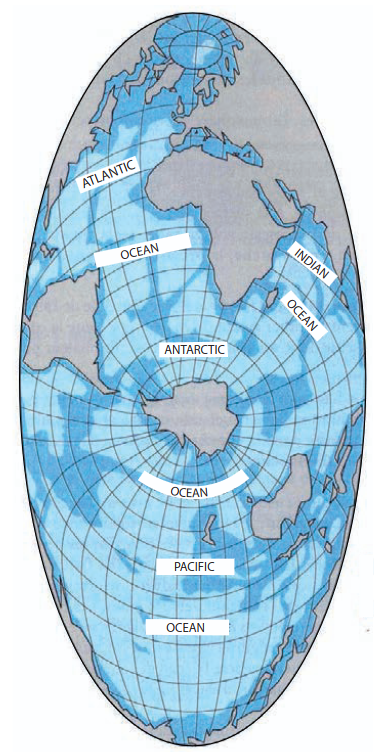
\includegraphics[width=0.3\textwidth]{images/intro/continuity_planteraryocean_fieux}
		\caption{Représentation des différents bassins océaniques et de leurs continuité.}
		\label{oceans}
	\end{figure}
	
	Un biotope correspond à l'espace physique et les conditions abiotiques associées dans lesquelles vit une biocénose. Une biocénose est l'ensemble des populations d'organismes qui occupent une zone donnée et interagissent entre elles. L'océan étant un milieu continu, seuls les paramètres physiques de l'eau (abiotiques) conditionnent la régionalisation en biotopes. La connaissance des paramètres physiques de l'eau est donc particulièrement importante pour l'étude des distribution des organismes et des niches écologiques marines. Les principaux paramètres abiotiques structurant les écosystèmes sont : la lumière (longueur d'onde et proportion d'éclairement), les propriétés hydrologiques (température et salinité) et l'hydrodynamisme. \textbf{il faut une source}. L'océan est stratifié verticalement selon la pénétration de la lumière : celle-ci dépendant de la profondeur. On parle de milieu eutrophe (épipélagique) entre 0 et 200m, de milieu dysphotique (mésopélagique) entre 200 et 1000m, de milieu aphotique (bathypélagique) entre 1000 et 4000m et de milieu abyssal au delà de cette dernière. Les propriétés hydrologiques de l'eau dépendent du climat : la chaleur et le vent induisent une évaporation rendant l'eau de mer plus salée, les précipitations induisent un adoucissement de la salinité. La composition chimique de l'eau de mer est fortement dépendante des apports du littoral (fer, nitrates, etc). L'hydrodynamisme inclue les marées et les divers courants induits par des gradients de température, de pressions. Ces derniers dépendent majoritairement du vent et de l'ensoleillement. La proximité au littoral participant grandement à la modification de ces paramètres abiotiques, on sépare l'océan horizontalement selon sa distance au plateau continental. On parle de zone pélagique au delà du plateau continental.
	
	L'écologie est une discipline qui s'intéresse aux interactions entre les différentes espèces d'un même biotope. Parmi elles, les relations trophiques (alimentaires) jouent un rôle fondamentale dans la structuration des écosystèmes. Dans le milieu océanique, le réseau trophique peut généralement être simplifié comme suis : 
	\begin{itemize} 	
		\item les producteurs primaires sont le phytoplancton
	\end{itemize}
	
	
	
	\subsection{L'Océan Austral}
	L'océan Austral (ou Antarctique) forme un anneau autour de l'Antarctide. Il représente 22\% de la surface totale des océans. Contrairement aux autres océans, iln'est pas délimité par des frontières continentales. En regardant une carte (voir figure \ref{label}), on pourrait penser qu'il est simplement la prolongation du bassin Atlantique, Pacifique et Indien. En réalité, il est délimité par une frontière océanographique : le Front Subtropical (approximativement à 40°S), caractérisé par de très forts gradients de températures. L'océan Austral se distingue également des autres océans par l'uniformité de son climat, de son hydrodynamisme et de ses propriétés hydrologiques.
	
	
	\subsection{Contexte Biologique}
	\subsubsection{Stratification Verticale}
	\subsubsection{Réseau Trophique}
	% plancton nekton etc
	
	
	\subsection{Contexte Physique}
	
	
	
	
	
	
	
	
	
	
	
	
	
	\section{Matériel}
	\subsection{Données Pigmentaires (PIGMeANN)}
	\subsection{Données hydrologiques (Copernicus)}
	\subsection{Données hydrodynamiques : FTLE}
	\subsection{Données d'acoustique active (OBSAUSTRAL)}
	
	\section{Méthode}
	\subsection{Pré-traitement des données}
	\subsubsection{Calcul des profils Sv moyens et du NASC}
	\subsubsection{Calcul des FOD}
	\subsubsection{Filtrage des pigments}
	\subsubsection{Colocalisation NASC/PIG/FTLE/FOD}
	\subsubsection{Diminution de l'autocorrelation spatio-temporelle}
	
	\subsection{Arbres de Régression}
	"Depending on the problem, the basic purpose of a classification/regression study can be either to produce an accurate classifier or to uncover the predictive structure of the problem." (classif. and regression trees p.6)
	Notre objectif ici est chercher à connaître la prédictibilié du NASC en fonction de la structure des communautés phytoplanctoniques, en lien avec l'activité de mésoéchelle. The goal is to understand the structural relationship between  the response and the measured variables. (p.221)
	
	\subsubsection{CART}
	
	\subsubsection{Random Forest}
	
	\subsubsection{Extreme Gradient Boosting}
	
	\section{Résultats}
	\subsection{Tendances inter-annuelles par FOD}
	\subsection{Résultats des régressions}
	
	\section{Résultats}
	
	\section{Discussion}
	
\end{document}